\documentclass[12pt]{report}

%Tous les packets
\usepackage{luatextra}
\usepackage{hyperref}
\usepackage{hhline}
\usepackage{multirow}
\usepackage{listings}
\usepackage{fancyhdr}
\usepackage[french]{babel}
\usepackage{lastpage}
\usepackage{amsmath}
\usepackage{float}
\usepackage[center]{caption}
\usepackage{enumitem}
%Page de garde
\title{Rapport Projet informatique 2020 :\\Site de rencontre}
\author{Nicolas \textsc{Bednarek} \and Théo \textsc{Julien} \and Julien \textsc{Richard}\and William \textsc{Kaczmarek}}
\date{20  avril au 21 juin 2020}
%Constantes pour tout le document
\usepackage[a4paper, left=1cm, right=1cm, top=2.5cm, bottom=2.5cm]{geometry}
\makeatletter
\let\theauthor\@author
\let\thetitle\@title
\makeatother

%Style du document entier
\pagestyle{fancy}
\renewcommand{\thesection}{\Roman{section}}
\fancyhead[R]{Site de rencontre}
\fancyhead[L]{CPI2 2019-2020}
\renewcommand\footrulewidth{1pt}
\fancyfoot[R]{\thepage /\pageref{LastPage}}
\fancyfoot[C]{}
\fancyfoot[L]{Bednarek, Julien, Kaczmarek, Richard}

\begin{document}
	\maketitle
	\tableofcontents
	\clearpage
\section{Introduction} 
	Pour terminer le module d'informatique cette année nous avons comme à notre habitude un projet de groupe à réaliser. Ce projet en groupe de 3 ou 4 étudiants, se déroule pendant 8 semaines environ. Laissant presque carte blanche à chaque groupe sur un thème sélectionnée. Nous avions à notre disposition 3 thèmes : \\
\begin{itemize}
	\item un site de services (du style AirBnB, Blablacar, etc...)
	\item un site rencontre
	\item un site d'e-commerce (Leboncoin, etc...)\\
\end{itemize}
Voulant avant tout s'amuser le plus possible, nous avons trouvé que le thème "site de rencontre" était le plus intéressant et avec le plus de défi.\\
\\
Nous devions tout d'abord trouver une spécificité à notre site. Nous avons voulu créer un site où l'authenticité était le principal point. Nous voulions à tout pris éviter les profils FAKE(=Faux), qui vendent des service externes et pollue l'application. Nous voulions aussi éviter que les gens mentent sur leur âges, en effet il est fréquent que des enfants ou adolescent s'inscrivent sur des applications en mentant sur leur âges. Ou encore des personnes se rajeunissant. Dans cette optique nous avons voulu réserver notre application aux étudiants, comme cela nous évitions les problèmes cité ci-dessus. En effet, en demandant la carte étudiante à l'inscription nous pouvions vérifier l'authenticité de la personne ainsi que son âge, même si celle-ci ment dessus si elle est étudiant elle sera forcément dans un tranche d'âges des autres utilisateurs. \\
\\ 
\begin{figure}[h!]
	\begin{center}
		
\includegraphics[scale=0.3]{intro.jpg}
	\end{center}
		\caption{Icone de différent site de recontre}
\end{figure}
\clearpage

\section{Notre projet/site}
	Quand on arrive pour la première fois sur notre site, on voit de suite deux boutons un pour la connexion et l'autre pour l'inscription. Nous avons fais le choix de ne pas permettre à un visiteur non inscrit de voir les profils de nos utilisateurs.
	\subsection{Inscription}
	Lorsqu'on clique sur se créer un compte une interface apparait permettant au visiteur de s'enregistrer. Pour cela il faut qu'il fournisse son : Nom, Prénom, Ville, adresse mail et enfin un mot de passe de compte qu'il devra confirmer.\\
	On remarque lorsqu'on commence à rentrer notre ville, au dessus de la zone une ville apparait selon les caractères inscrit. C'est l'API d'adresse du gouvernement français qui détecte la ville, cela nous permet de récupérer la position exact du visiteur afin de savoir à combien de km le séparera des autres profils.\\
On remarque aussi que lorsqu'on commence à taper notre mot de passe une barre de couleur apparait en dessous, cela est la force de notre mot de passe. Une fois toutes les données entrées on clique sur "s'enregistrer". Si tout va bien, une nouvelle interface apparait nous indiquant que notre compte à bien été crée, et nous propose alors d'envoyer notre carte étudiante cette étape permet de vérifier notre compte. Cette carte étudiante ne doit pas dépasser 2 Mo, et peut être au format .png/.jpg/.jpeg.\\
Si l'on upload notre carte la création du compte est terminée , dans le cas où l'on upload pas notre carte nous pouvons quand même nous connecter et dans notre profil on pourra upload notre carte étudiante.
\subsection{Connexion}
	Lorsqu'on clique sur le bouton connexion une interface classique de connexion apparait pour nous connecter. Une fois connecter on apparait directement sur l'interface principale.
\begin{figure}[h!]
	\begin{center}
		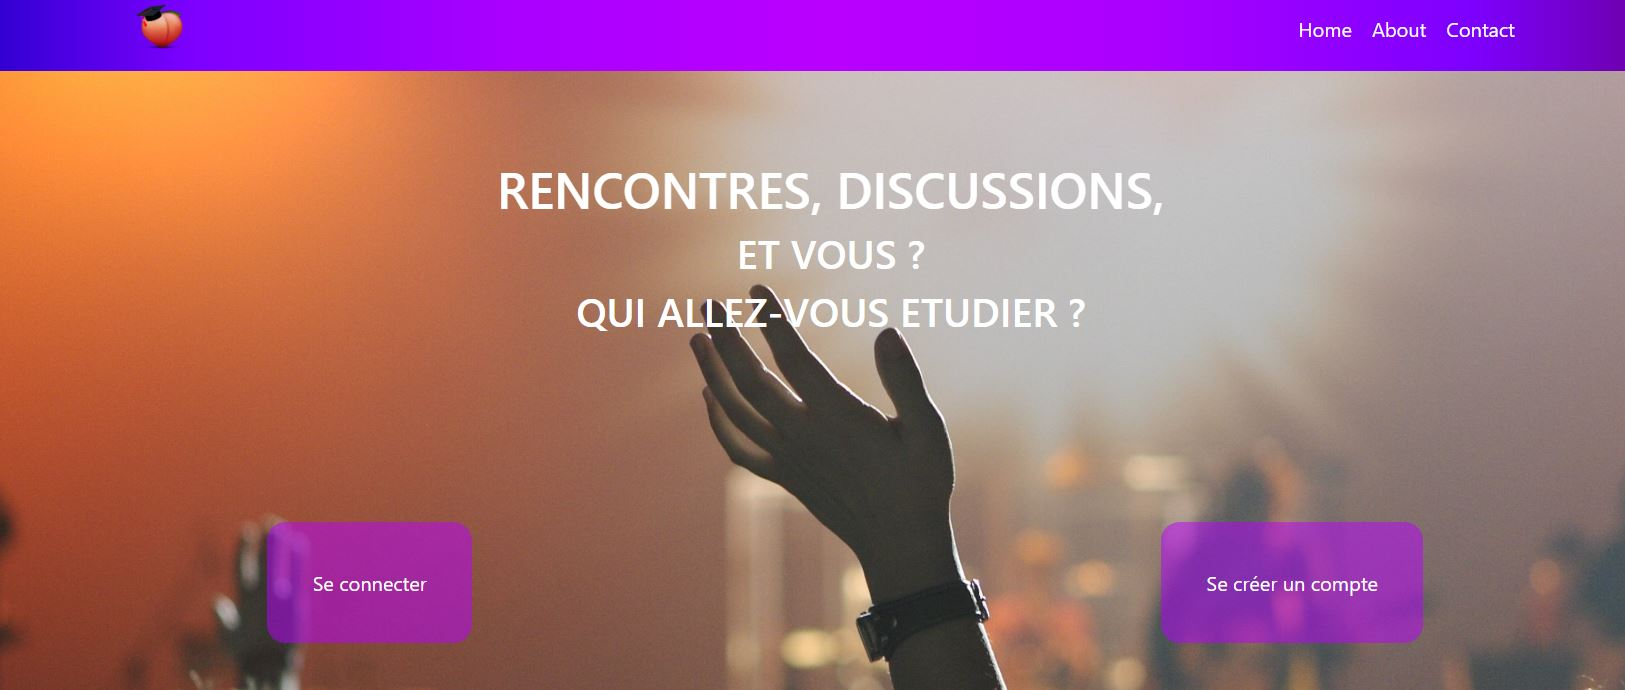
\includegraphics[scale=0.5]{acceuil.jpg}
	\end{center}
		\caption{Capture d'écran de notre site}
\end{figure}
\clearpage
\subsection{Acceuil}
\begin{figure}[h!]
	\begin{center}
		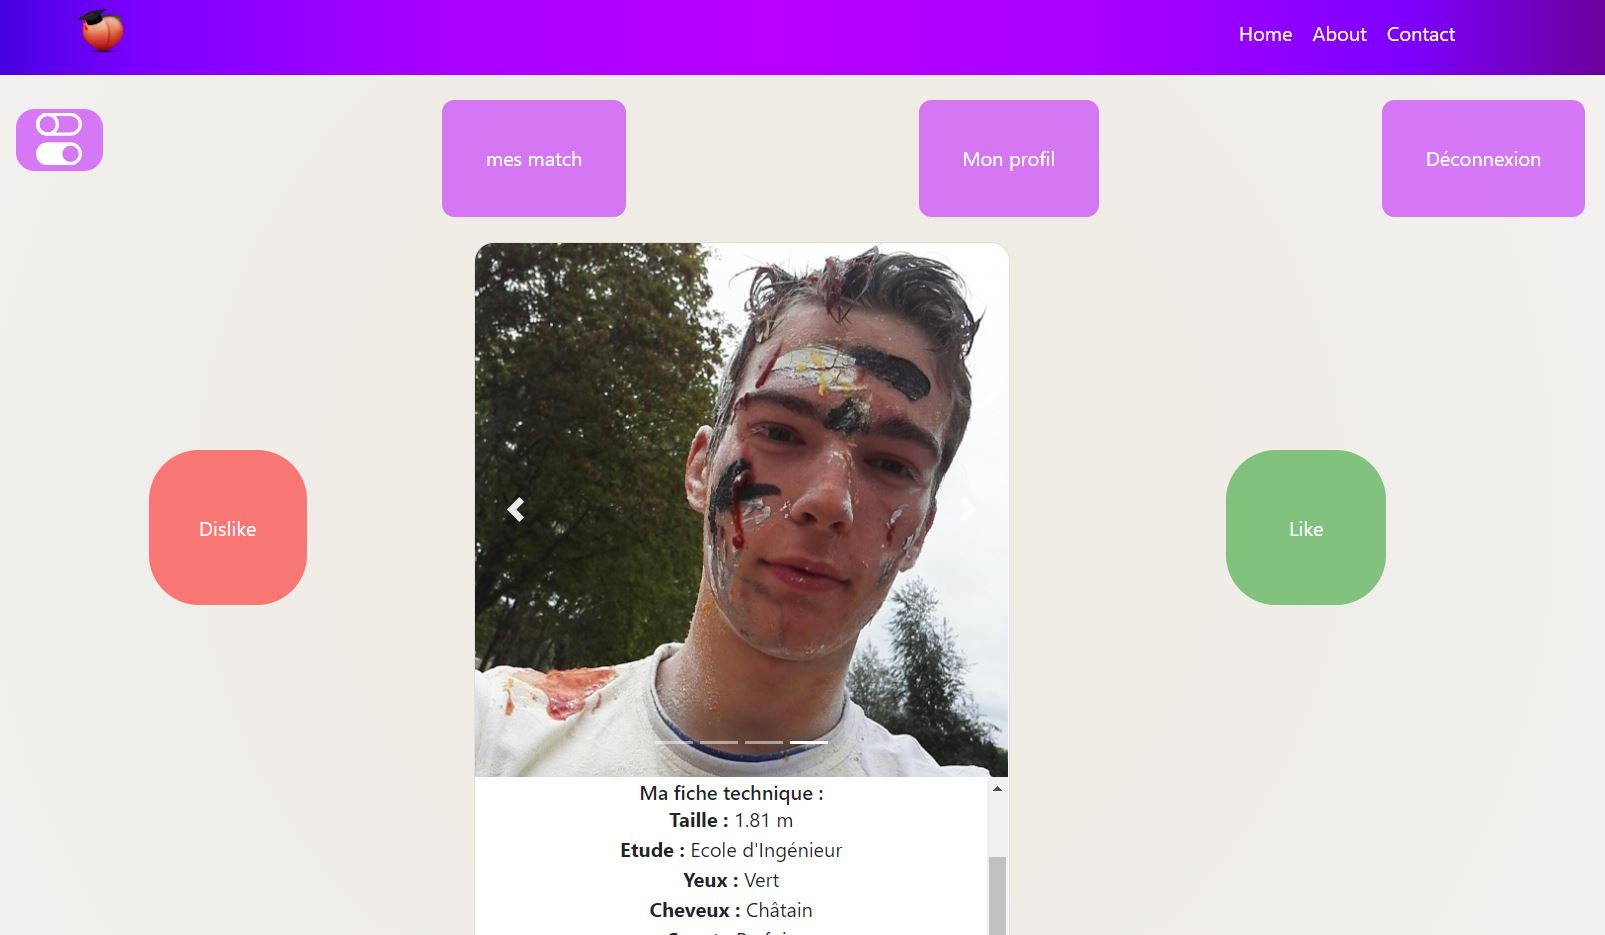
\includegraphics[scale=0.5]{principal.jpg}
	\end{center}
		\caption{Capture d'écran de notre site une fois connecté}
\end{figure}
Nous voila enfin sur la page principal on peut y voir les profils des autres utilisateurs selon les paramètres défini, l'on peut les likes ou les dislikes. Pour modifier ses paramètres, il suffit de cliquer sur le bouton "Mon profil", on accèdera alors à la page permettant de gérer son profil, ou l'on peut ajouter nos photos, une description ainsi que ajouter pleins d'informations nous concernant tel que la couleur de nos yeux, si l'on possède des animaux de compagnie ou encore si nous sommes fumeur.\\
Le bouton match, permet d'accéder à nos match, c'est a dire si l'une personne qui nous avons liké, nous a liké en retour. Dans cette page l'on peut notamment accéder à notre messagerie et ainsi discuter avec nos matchs.
\\
Le dernier boutons intéressant est le bouton tout en haut à gauche, celui-ci permet d'accéder aux filtres afin d'affiner nos recherches. En effet avec les filtres on peut choisir de ne voir que les profils correspondant à ses attentes, par exemple si l'on souhaite rencontrer que des non-fumeurs ce sera ici qu'il faudra le gérer. Cet option est toutefois réservé au membre premium. Il faut donc s'abonner afin de bénéficier de ce service.
\clearpage
\subsection{NavBar}
	En haut du notre site on peut voir une NavBar avec notre icone ainsi que trois boutons : \\
	\begin{itemize}
		\item Home
		\item About us
		\item Contact
	\end{itemize}
Le bouton home permet de revenir sur la page de connexion si on n'est pas connecté au site, et permet de retourner sur la page principal si l'on est connecté.\\
Le bouton About us, affiche la même page que l'on soit connecté ou pas à notre site. Cette page présente chacun des membres du projet.\\
Enfin le bouton Contact, tout comme About us est accessible qu'on soit connecté ou pas, cette page permet de contacter les administrateurs du site par mail.
\begin{figure}[h!]
	\begin{center}
		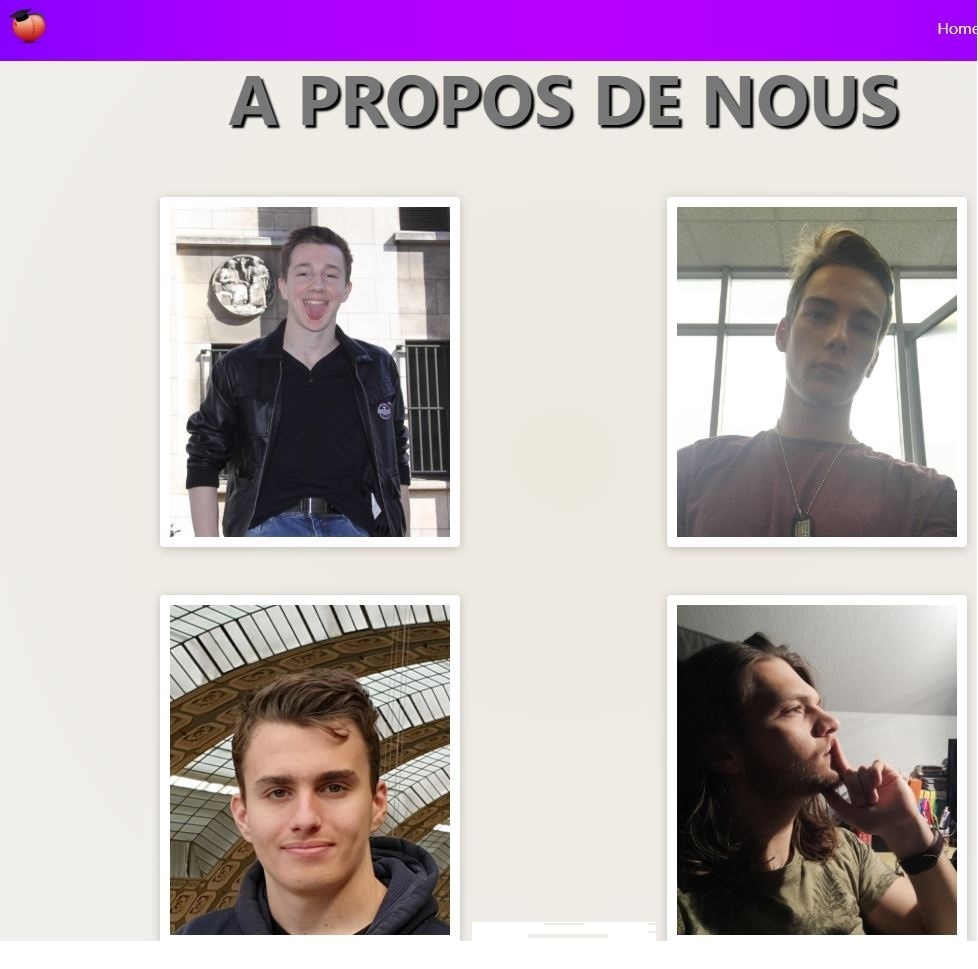
\includegraphics[scale=0.5]{Aboutus.jpg}
	\end{center}
		\caption{Capture d'écran de notre site une fois connecté}
\end{figure}
\clearpage
\section{Nos objectifs et les perspectives d'avenir}
	
\section{Conclusion de ce projet}

			\begin{thebibliography}{10}
			\bibitem{HTTP}
			Définition HTTP
			\emph{https://developer.mozilla.org/fr/docs/Web/HTTP}
			
		\end{thebibliography}
\end{document}
